\documentclass[a4paper,11pt]{report}
\usepackage[french]{babel}
\usepackage[T1]{fontenc}
\usepackage[utf8]{inputenc}
\usepackage{lmodern}
\usepackage{microtype}
\usepackage{hyperref}
\usepackage{tabulary}
\usepackage{framed}
\usepackage{fancyhdr}
\usepackage{amsmath}
\usepackage{bbm}
\usepackage{graphicx}
%\usepackage{pst-all}
%\usepackage{xcolor}
%\usepackage{nopageno}

%\newcommand{\latin}[1]{\textit{#1}}

\usepackage[margin=1.0in]{geometry}

%%%%%%%%%%%%%%
%\usepackage{geometry}
 %\geometry{
% a4paper,
 %total={210mm,297mm},
 %left=20mm,
 %right=20mm,
 %top=20mm,
 %bottom=20mm,
 %}
 %%%%%%%%%%%%%%
 
\pagestyle{empty}

\pagestyle{fancy}
\fancyhead{}
\renewcommand{\headrulewidth}{0.5pt}
\fancyhead[R]{\textit{\nouppercase{\rightmark}}}
\fancyfoot{}
\renewcommand{\footrulewidth}{0.5pt}
\fancyfoot[L]{\textit{\nouppercase{\leftmark}}}
\fancyfoot[R]{\thepage}
  
\begin{document}
	\begin{titlepage}
		\vspace*{\stretch{2}}
		\begin{center}
			\large\bfseries\itshape Stage ETE 2015\\
		\end{center}
		\noindent\rule{\linewidth}{3pt}

		\begin{center}
			\Huge\bfseries\itshape Description du système\\
		\end{center}
		
		\noindent\rule{\linewidth}{3pt}
		\begin{center}
			\bfseries
			\large F-PHT \\
			\large Un système d'index de filtres de Bloom pour la recherche d'information par mots clés
		\end{center}
		\vspace*{\stretch{2}}
		\begin{center}
			Réalisé par \textbf{DOAN} Cao Sang \\
			Encadrant: M. \textbf{MAKPANGOU} Mesaac, Regal
		\end{center}
		\vspace*{\stretch{0.5}}
		\begin{center}
			1 Juillet 2015
		\end{center}
	\end{titlepage}

\tableofcontents

\chapter{Vue globale}
\section{Prefix Hash Tree (PHT)}
	Un arbre préfixe est un arbre numérique ordonné qui est utilisé pour stocker une table associative où les clés sont généralement des chaînes de caractères. Contrairement à un arbre binaire de recherche, aucun nœud dans le trie ne stocke la chaîne à laquelle il est associé. C'est la position du nœud dans l'arbre qui détermine la chaîne correspondante\footnote{Wikipédia}.
	
	Pour tout nœud, ses descendants ont en commun le même préfixe. La racine est associée à la chaîne vide. Des valeurs ne sont pas attribuées à chaque nœud, mais uniquement aux feuilles et à certains nœuds internes se trouvant à une position qui désigne l'intégralité d'une chaîne correspondante à une clé.
	
	Pour faire une recherche d'une valeur associée à une clé, au départ, on se situe à la racine de l'arbre, en prenant le premier élément de la clé de la requête, on trouve le chemin étiqueté par cet élément, s'il n'existe pas, on est sûr que cette clé n'est pas dans l'arbre. Dès que l'on trouve le chemin, on arrive sur le bon nœud et continue en prenant le deuxième élément de la clé de requête, on applique cette méthode jusqu'à quand on trouve cette clé et se termine sur une feuille.
	
	\begin{figure}[!htbp]
	\centering
	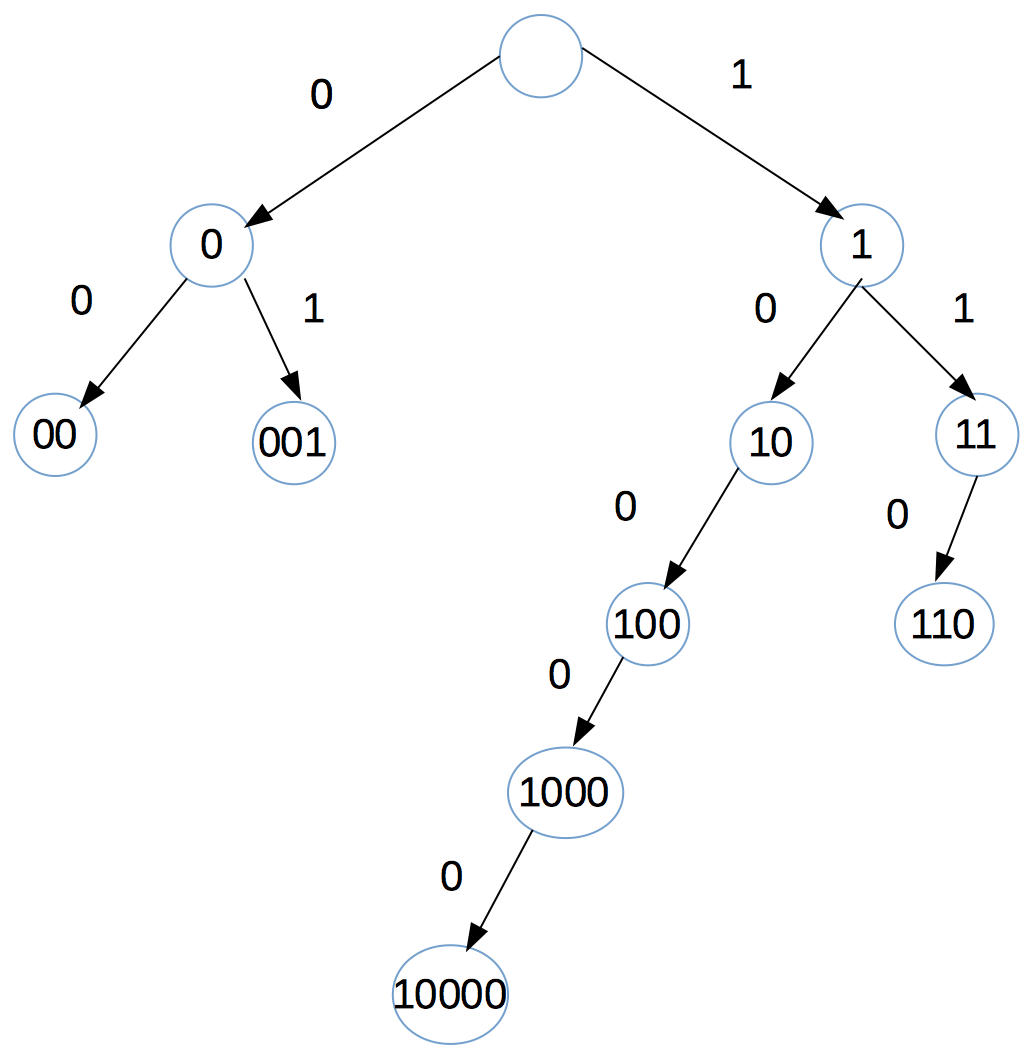
\includegraphics[width=12cm]{PHT.eps}
	\caption{Arbre de préfixe}
	\label{PHT}
	\end{figure}	

\newpage	
	
\section{F-PHT}
	F-PHT est un arbre préfixe de "multibit". Pour stocker une clé, on suit le chemin étiqueté par les fragments successifs de cette clé (dans l'ordre de leur rang) jusqu'à ce qu'on arrive sur une feuille pouvant stocker cette clé.

	Un fragment est un morceau d'une clé (sous-ensemble de bits). Si on considère les clés de taille \textit{m}, le système découpe chaque clé en \textit{f} fragments de taille identique. Par convention, ces fragments sont numérotés de \textit{0} à \textit{f-1}.
	
	\begin{table}[!h]
		\centering		
		\begin{tabular}{|l|*{14}{c|}r|}
		\multicolumn{1}{c}{{\scriptsize 15}} &\multicolumn{1}{c}{}&\multicolumn{1}{c}{}&\multicolumn{1}{c}{}&
		\multicolumn{1}{c}{}&\multicolumn{1}{c}{}&\multicolumn{1}{c}{}&\multicolumn{1}{c}{}&
		\multicolumn{1}{c}{}&\multicolumn{1}{c}{}&\multicolumn{1}{c}{}&\multicolumn{1}{c}{}&
		\multicolumn{1}{c}{}&\multicolumn{1}{c}{}&\multicolumn{1}{c}{}&\multicolumn{1}{c}{{\scriptsize 0}}\\
		\hline
			1 & 0 & 0 & \multicolumn{1}{c||}{0} & 
			1 & 1 & 0 & \multicolumn{1}{c||}{1} & 
			0 & 0 & 0 & \multicolumn{1}{c||}{0} & 
			1 & 0 & 1 & 0 \\
		\hline
		\end{tabular}
		\caption{Exemple le filtre de Bloom}
		\label{fragment/filtredeBloom}
	\end{table}
	
	La table \ref{fragment/filtredeBloom} représente une clé de taille \textit{m = 16} bits, elle est ensuite découpée en \textit{f = 4} fragments. Le premier fragment est la suite de bits \textit{"1000"} qui se trouve les plus à gauche de cette clé. Le dernier est \textit{"1010"}.
	
	\begin{figure}[!htbp]
	\centering
	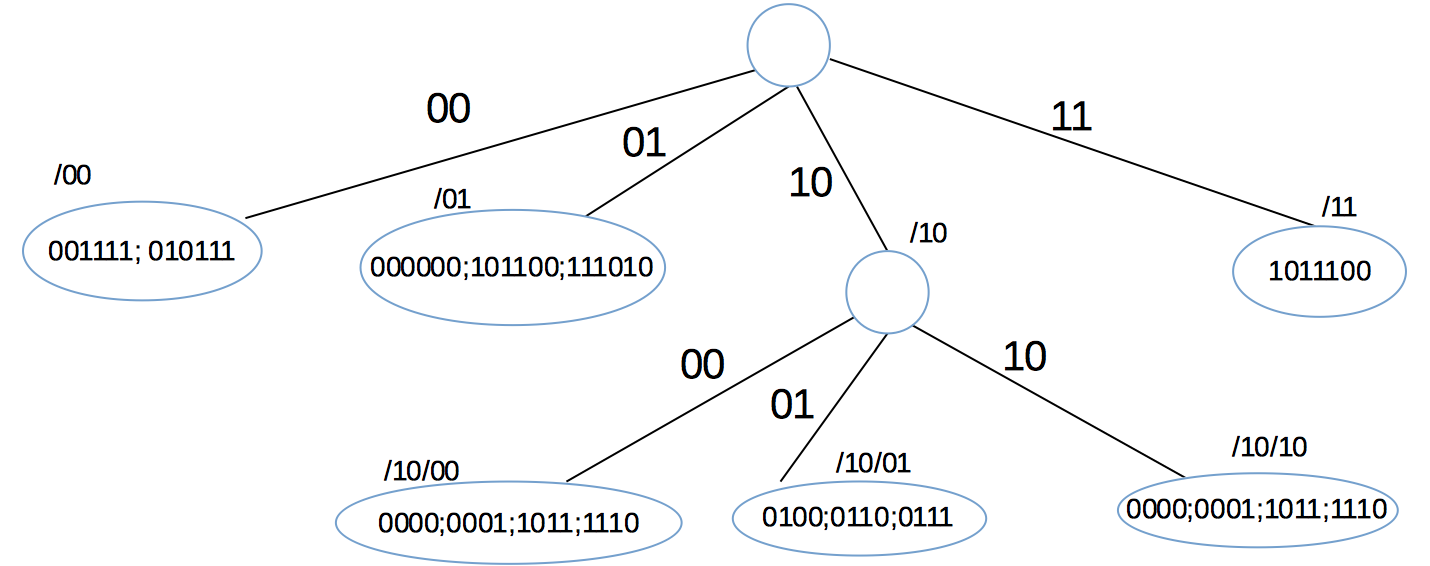
\includegraphics[scale=0.70]{F-PHT_2.eps}
	\caption{Arbre F-PHT}
	\label{F-PHT2}
	\end{figure}	
	
	La figure \ref{F-PHT2} représente l'arbre F-PHT qui stocke une clé de taille \textit{m = 8} bits, la taille d'un fragment est de 2 bits. Au dessus de chaque nœud (interne ou feuille) se trouve son identifiant unique et il caractérise également le chemin unique qui conduit vers ce nœud.
	
\chapter{Système d'indexation}
\section{Objectif}
	Les clés indexées sont des filtres de Bloom de taille \textit{m}.
	L'objectif du système est d'une part de stocker les filtres de Bloom donnés par les utilisateurs, d'autre part de permettre de rechercher tous les filtres de Bloom (stockés dans le système) qui sont sur-ensemble d'un filtre de Bloom caractérisant des mots clés d'une requête.

\section{Architecture du système d'indexation}
	Le système d'indexation est réalisé par un ensemble de serveurs d'index répartis sur plusieurs machines. Chaque serveur gère un ou plusieurs nœuds de l'arbre F-PHT. Ce système permet de créer plusieurs index, chaque index maintient  un F-PHT qui stocke les clés.
	
	On suppose qu'il y a un serveur central connu qui gère tous les index créés. Il utilise une table des index, chaque entrée sert à sauvegarder l'identifiant de l'index \textit{indexID} et le serveur \textit{rootNodeID} qui héberge sa racine. Lorsqu'un utilisateur veut créer/supprimer un index, il demande le serveur central d'ajout/suppression une entrée dans la table des index.

\section{API du système d'indexation}
	Ce système offre aux utilisateurs des services suivants :
	\begin{description}
		\item[	createIndex() 	 :] créer un nouveau index et rend aux l'utilisateur l'identifiant d'index créé \textit{indexID}.
		\item[	removeIndex(indexID)	 :] supprime un index identifié par \textit{indexID}.
		\item[	add(indexID, key) 		 :] ajoute dans l'index identifié par \textit{indexID} une clé \textit{key}.
		\item[	remove(indexID, key)  :] supprime une clé \textit{key} dans l'index identifié par \textit{indexID}.
		\item[	search(indexID, key\_req) 	 :] recherche dans l'index identifié par \textit{indexID} des sur-ensembles qui satisfont la requête \textit{key\_req}.
	\end{description}

	
\chapter{Fonctionnement du système}
\section{Données de chaque nœud dans l'arbre}
	\begin{description}
		\item[Identifiant d'un nœud] caractérise le nœud. Cet identifiant est calculé grâce au chemin vers ce nœud, et ce chemin est unique.
		\item[Niveau d'un nœud (rang)]  est l'hauteur dans l'arbre F-PHT.
		\item[Table de routage (LocalRoute)] sert :
			\begin{itemize}
				\item soit à router chaque requête vers le nœud fils responsable de la traiter.
				\item soit à déterminer l'adresse du conteneur local. Ce conteneur stocke au maximum $\gamma$ éléments.
			\end{itemize}
	\end{description}


\section{Protocole}
\subsection{Ajout d'un filtre de Bloom dans F-PHT}
	Lorsqu'un nœud reçoit une requête d'ajout d'un filtre de Bloom (c'est-à-dire d'une clé), il effectue deux actions :
	\begin{enumerate}
		\item Premièrement, il détermine la valeur du fragment numéro \textit{i} de la clé à ajoutée, avec \textit{i} correspondant au niveau de ce nœud dans l'arbre F-PHT.
		\item Une fois le fragment de la clé de rang \textit{i} déterminé, il consulte l'entrée de la table de routage \textit{LocalRoute} associée à cette valeur. Trois cas sont à distinguer :
		\begin{enumerate}
			\item Si l'entrée est nulle (aucune clé ayant la même valeur pour le fragment de rang \textit{i} a été ajoutée auparavant), le nœud crée un conteneur local, ajoute son adresse dans cette entrée et stocke la clé reçue dans ce conteneur.
			\item Si l'entrée associée à la valeur du fragment de rang \textit{i} contient l'identifiant d'un nœud fils, on transmet la requête vers ce fils.
			\item Si l'entrée contient l'adresse d'un conteneur local, on ajoute la clé reçue dans ce conteneur. Si après ajout, le nombre d'éléments stockés dépasse le seuil fixé, le nœud crée un nœud fils, lui transmet le conteneur, et met à jour l'entrée correspondante l'adresse de son nouveau fils.
		\end{enumerate}
	\end{enumerate}
		
\subsection{Recherche des filtres de Bloom dans F-PHT}
	Lorsqu'un nœud reçoit une requête de recherche des sur-ensembles d'un filtre de Bloom, il effectue les étapes suivantes :
	\begin{enumerate}
		\item D'abord, il détermine la valeur du fragment numéro \textit{i} de la clé de requête, avec \textit{i} correspondant au niveau de ce nœud dans l'arbre F-PHT.
		\item Ensuite, il consulte toutes les entrées de la table de routage \textit{LocalRoute} contiennent la valeur du fragment déterminée précédente. Pour chaque entrée, il y a 3 cas à traiter :
		\begin{enumerate}
			\item Si l'entrée est nulle (aucune clé contenant cette valeur du fragment de rang \textit{i}), le nœud continue.
			\item Si l'entrée associée à la valeur du fragment de rang \textit{i} contient l'identifiant d'un nœud fils, on transmet la requête vers ce fils.
			\item Si l'entrée contient l'adresse d'un conteneur local, on collecte tous les filtres qui contiennent la requête. L'ensemble des filtres collectés est retourné comme réponse.
		\end{enumerate}
		\item Puis, il attend toutes les réponses des fils auxquels il ont transmis la requête. Une fois, il reçoit toutes les réponses et réunit avec son ensemble des résultats, il transmet le résultat au père.
	\end{enumerate}
	
\subsection{Suppression d'un filtre de Bloom dans F-PHT}
	Les étapes de la suppression d'un filtre de Bloom dans F-PHT effectuées par un nœud sont :
	\begin{enumerate}
		\item Il détermine la valeur du fragment numéro \textit{i} de la clé de requête, avec \textit{i} correspondant au niveau de ce nœud dans l'arbre F-PHT.
		\item Ensuite, il consulte l'entrée de la table de routage \textit{LocalRoute} associée à cette valeur. Trois cas sont à distinguer :
		\begin{enumerate}
			\item Si l'entrée est null (aucune clé ayant la même valeur pour le frament numéro \textit{i} a été ajoutée auparavant), le nœud rejette la requête.
			\item Si l'entrée associée à la valeur du fragment de rang \textit{i} contient l'identifiant d'un nœud fils, on transmet la requête vers ce fils.
			\item Si l'entrée contient l'adresse d'un conteneur local, on supprime la clé de requête dans ce conteneur. Si après suppression, ce conteneur devient vide, on supprime ce conteneur et cette entrée dans la table \textit{LocalRoute}. Si cette table devient vide, il notifie le père de la suppression de son fils et demande le système de supprimer ce nœud. Si le père reçoit la notification de son fils, il vide l'entrée où stocke son adresse. En plus, si la table de routage \textit{LocalRoute} de son père devient aussi vide, il fait la même procédure comme son fils : notifie son père, demande la suppression du système.
		\end{enumerate}
	\end{enumerate}

\chapter{Implémentation du système}
\section{Plateforme de simulation}
	Cette plateforme est destinée à simuler le système d'indexation, dans un premier temps, il est centralisé sur une seule machine. Elle crée un index, ensuite ajoute des données dans cet index. A la fin, une suite de requête de recherche des données est lancée pour tester le fonctionnement du système. Elle peut également simuler la suppression des données dans le système.
	
	Le simulateur maintient une table des des instances de serveurs existants dans ce système, il joue aussi le serveur de localisation des index.
	
	L'application interagit avec le système via l'API.
	
\section{Serveur}
	Les serveurs se communique via une interface de réseau qui permet d'envoyer et recevoir des messages.
	
\section{Implémentation du système}
	

\end{document}









